\documentclass[sigconf,nonacm]{acmart}
\settopmatter{printacmref=false,printfolios=true}
\setcopyright{none}
\renewcommand\footnotetextcopyrightpermission[1]{}
\usepackage{amsmath,tabularx,array,enumitem,balance,tikz,graphicx}
\usetikzlibrary{arrows.meta,positioning,shapes.geometric}
\definecolor{CourseBlue}{HTML}{315EFB}
\definecolor{CourseTeal}{HTML}{14877D}
\definecolor{CourseInk}{HTML}{18324A}
\hypersetup{colorlinks=true,linkcolor=CourseBlue,citecolor=CourseTeal,urlcolor=CourseTeal}
\newcolumntype{Y}{>{\raggedright\arraybackslash}X}
\setlist{leftmargin=*,topsep=3pt,itemsep=2pt}
\newcommand{\CourseNumber}{COMSCI/ECON 206}
\newcommand{\CourseName}{Computational Microeconomics}
\newcommand{\CourseSession}{Autumn 2026 Session 1}
\newcommand{\Instructor}{Professor Luyao Zhang}
\newcommand{\TeamCode}{Team7}
\newcommand{\SymposiumSession}{A}
\newcommand{\GitHubLink}{\url{https://github.com/z2005lin/PS2_Zijie_Lin}}
\newcommand{\NotebookLink}{\url{https://colab.research.google.com/drive/1Ox65uxV-g7nPSgpChWZFGmYOfYQTQoCi?usp=sharing}}
\newcommand{\HuggingFaceLink}{\url{https://huggingface.co/spaces/dku-comsci-econ206-2026/SubmitOrWait}}
\newcommand{\PosterLink}{Draft figure: \texttt{figures/fee\_choice\_teaser.pdf}; A0 poster not yet available}
\newcommand{\coursemeta}{\noindent\textbf{Submission to:} \CourseNumber{} --- \CourseName.\\
\textbf{Course session:} \CourseSession. \textbf{Team:} \TeamCode. \textbf{Symposium:} \SymposiumSession.\\
\textbf{Course instructor:} \Instructor. \textbf{Assignment:} PS2 collaborative research proposal.\par\smallskip}
\title{Strategic Fee-Level Choice under Incomplete Information: An Anti-Coordination Game on Algorand}
\author{Lin Zhang}
\affiliation{\institution{Duke Kunshan University}\city{Kunshan}\country{China}}
\email{lin.zhang@dukekunshan.edu.cn}
\author{Zijie Wang}
\affiliation{\institution{Duke Kunshan University}\city{Kunshan}\country{China}}
\email{zijie.wang@dukekunshan.edu.cn}
\renewcommand{\shortauthors}{Team7}

% The instructor is course metadata, not a paper author.

\begin{document}
\begin{teaserfigure}
\captionsetup{skip=8pt}
\centering
% Proposal-specific teaser shown at its original aspect ratio with no cropping.
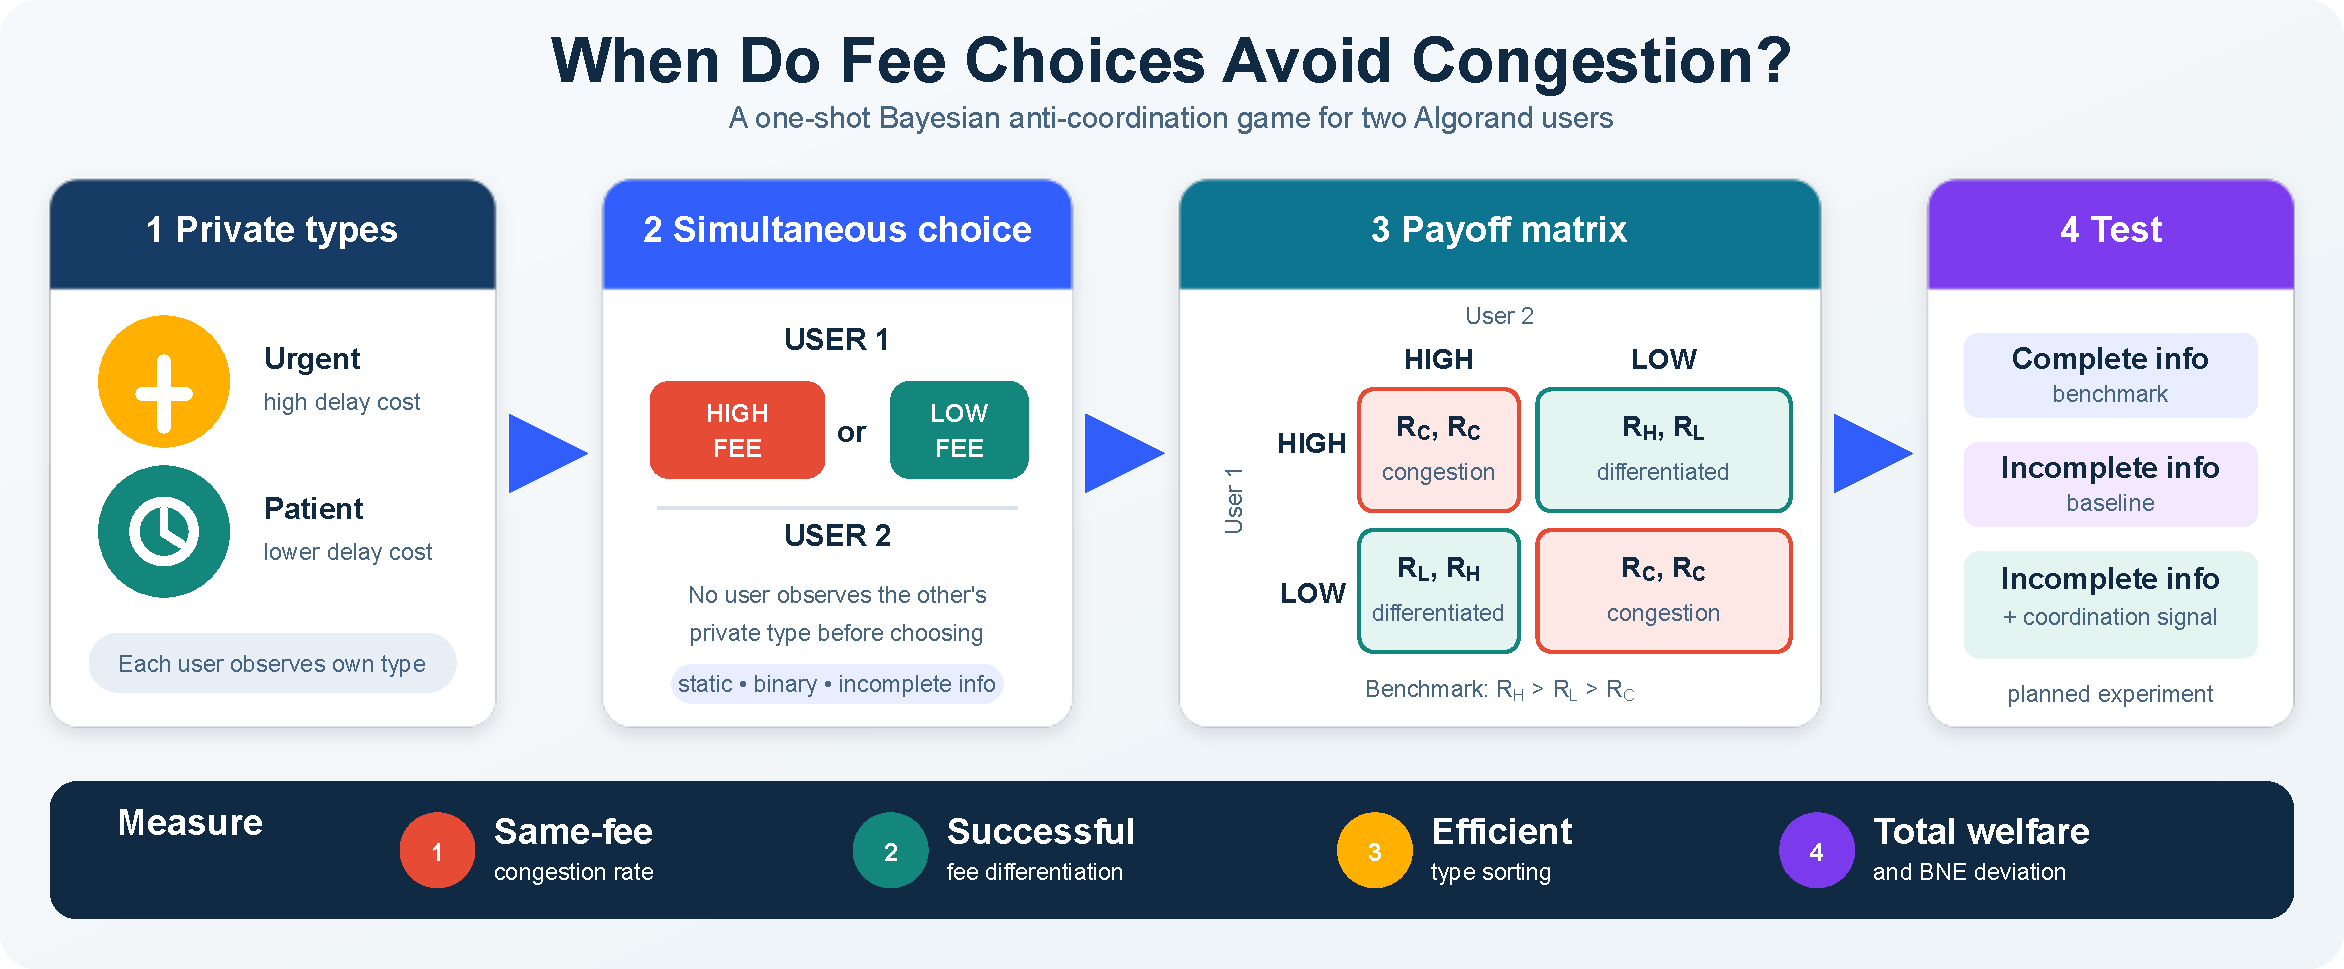
\includegraphics[width=\textwidth]{figures/fee_choice_teaser.pdf}

\caption{Research design for a one-shot Bayesian anti-coordination game. Two privately informed users simultaneously choose High or Low fees; the matrix identifies congestion and differentiated outcomes, and three treatments test how information and coordination signals affect behavior and welfare. All arrows from treatments to outcomes represent planned tests, not reported results.}
\Description{Private urgency types lead two users to simultaneous High or Low fee choices. A payoff matrix distinguishes same-fee congestion from successful fee differentiation. Complete information, incomplete information, and signal treatments are compared using congestion, sorting, and welfare outcomes.}
\label{fig:teaser}
\end{teaserfigure}
\maketitle\raggedbottom\coursemeta

\noindent\textcolor{CourseTeal}{\textbf{PS1-continuous template.}} This file retains the required PS1 ACM layout, five-section main paper, Author Notes, references, and Appendices A--E. Appendix F contains the additional PS2 experiment, linked-artifact, poster, and symposium records. The repository and behavioral demo are implemented; numerical notebook outputs are simulated, and no laboratory result is reported.

\section{Three connected research questions and verified gap}
Blockchain fee mechanisms allocate scarce inclusion capacity~\cite{roughgarden2024}, while Algorand supplies the protocol setting~\cite{gilad2017}. We study its smallest strategic fee-choice abstraction: two privately informed users simultaneously choose \emph{High} ($H$) or \emph{Low} ($L$). Equal choices create congestion and low rewards; different choices avoid the conflict. This is a one-shot static Bayesian anti-coordination game connecting equilibrium analysis, information design, and behavioral measurement.

\textbf{Q1---Economics:} How do private urgency and value affect coordination and welfare? \textbf{Q2---Computation:} Which pure, mixed, and Bayesian equilibria follow from explicit payoffs and type beliefs? \textbf{Q3---Behavior:} Does incomplete information increase same-fee failure, and can a signal reduce it? Figure~\ref{fig:teaser} connects types, choices, matrix outcomes, treatments, and metrics.

\section{Answer to Q1: incentives and strategic model}
Users $i\in\{1,2\}$ privately observe type $\theta_i\in\{U,P\}$ (urgent or patient) and simultaneously choose $a_i\in\{H,L\}$. Conditional on types,
\[
\begin{array}{c|cc}&H&L\\\hline H&(R_C,R_C)&(R_H,R_L)\\L&(R_L,R_H)&(R_C,R_C)\end{array}
\]
where $R_C$ is the same-fee congestion reward. If $R_H>R_L>R_C$, $(H,L)$ and $(L,H)$ are pure Nash equilibria~\cite{nash1950}; the symmetric mixed equilibrium chooses $H$ with $p^*=(R_H-R_C)/(R_H+R_L-2R_C)$. With private types, payoffs become type-dependent and the solution is Bayesian Nash equilibrium~\cite{harsanyi1968}. Solving it requires a type prior and type-specific payoffs, which remain calibration inputs.

\textbf{Game theory} characterizes best responses; \textbf{social choice} compares equilibrium with the welfare-maximizing assignment of one user to each fee; \textbf{mechanism design} asks whether a feasible recommendation can improve coordination without revealing types, drawing on correlated equilibrium and information design~\cite{aumann1974,bergemann2016}.

\section{Answer to Q2: computation, auction comparison, and artifacts}
The computational implementation and planned human experiment follow induced-value principles~\cite{smith1976} and compare: (1) complete information; (2) incomplete information; and (3) incomplete information plus a coordination signal. Participants would be randomly rematched across one-shot rounds. Outcomes are same-fee congestion, differentiation, urgent-user selection of $H$, welfare, and deviation from Bayesian equilibrium. The design builds on experimental evidence about strategic uncertainty, focal points, and asymmetric coordination signals~\cite{vanhuyck1990,crawford2008,agranov2012}. Notebook outputs are conditional simulations; all human treatment effects remain hypotheses.

The scarce resource is differentiated transaction priority. This is not a full auction: choices are binary, and continuous bids, endogenous payments, and seller revenue are absent. Algorand fee and confirmation mappings, empirical payoffs, type probabilities, human sample size, and statistical tests must be calibrated or preregistered before a laboratory implementation.

\textbf{Computational scientist---GitHub:} \GitHubLink\\
\textbf{Runnable notebook:} \NotebookLink\\
\textbf{Behavioral scientist---Hugging Face:} \HuggingFaceLink\\
\textbf{Interdisciplinary scholar---A0 poster:} \PosterLink

\clearpage\balance
\section{Answer to Q3: behavior and interdisciplinary integration}
The rational benchmark assumes correct beliefs and payoff maximization. Alternatives include level-$k$ reasoning, focal attraction, ambiguity aversion, and reinforcement~\cite{camerer2003,zhu2025}. Treatment choices and elicited beliefs will distinguish them: convergence to type-dependent best responses supports the benchmark; persistent same-fee clustering after beliefs stabilize motivates revision. The current Hugging Face artifact is an exploratory behavioral interface with simulated co-players; no participant dataset currently exists.

\section{Advanced development, real-world impact, and roadmap}
The project connects Nash and Harsanyi foundations to a reproducible blockchain fee-choice experiment. Users, wallet designers, and protocol researchers could benefit from validated evidence about fee-menu or recommendation design. Risks are unrepresentative payoffs and treating a two-user laboratory game as a live-network model. Value therefore requires documented Algorand mapping, open code, robustness, and type-specific welfare checks. Academia requires identification and replication; industry adds operational tests; public institutions require accessibility and accountability. The next test is whether incomplete information causally raises same-fee congestion.

\begin{table}[h]\caption{From foundations to a collaborative interdisciplinary contribution.}
\begin{tabularx}{\columnwidth}{@{}p{1.6cm}Y@{}}\toprule
\textbf{Horizon}&\textbf{Milestone and evidence}\\\midrule
Foundation&Static $H/L$ game and equilibrium concepts.\\
PS2&Model, teaser, treatments, open code, and conditional simulated outputs; no empirical result.\\
Symposium&Planned poster, peer challenge, and response.\\
Next study&Calibration, preregistration, and human experiment.\\
2056&Accountable coordination tools for transaction markets.\\\bottomrule
\end{tabularx}\end{table}

\noindent\textbf{Expected 2056 Nobel Prize and Turing Award contribution statement.}
By 2056, we aspire to develop theory and auditable tools for coordination under private transaction urgency. Progress would require replicated experiments, field validation, open implementation, and independently verified welfare gains.

\subsection*{Open Science Statement}
Lin Zhang created the GitHub, notebook/Colab, and Hugging Face artifacts. The repository records URLs, license, parameters, seeds, commands, simulated outputs, and limitations. Zijie Wang will prepare the editable A0 poster.

\subsection*{Statement of Contribution to the UN's SDGs}
No SDG impact is demonstrated. A future SDG 9 claim requires evidence that the mechanism improves reliable access without disadvantaging patient or lower-value users.

\subsection*{Submission milestones}
Review-ready: September 27, 2026, 11:00 P.M. Beijing time. Symposium: September 28, 2026, 2:45--5:15 P.M., IB 2050. Final revision: September 30, 2026, 11:00 P.M. Beijing time.

\clearpage\nobalance
\section*{Author Notes}
\subsection*{Acknowledgements}
\textbf{Course instructor: Professor Luyao Zhang.} We acknowledge OpenAI Codex for assistance on September 25--27, 2026 with transferring the authors' proposal into the required LaTeX structure, refining the teaser figure, organizing the repository, and checking layout. No empirical result was generated or verified by this assistance. No peer, discussant, community, or industry feedback has yet been received. The authors remain responsible for every claim, citation, computation, and remaining error.

\subsection*{Team and individual contributions}
Team 7 jointly narrowed the study to a two-user High/Low fee-choice game and specified the equilibrium and experiment plan. \textbf{Lin Zhang} implemented the GitHub repository, runnable notebook/Colab, and Hugging Face behavioral artifact. \textbf{Zijie Wang} developed the proposal and Overleaf submission, coordinated the model framing and teaser, and will produce the A0 poster. Both authors will calibrate the game, verify outputs, interpret results, and revise claims after feedback.

\bibliographystyle{ACM-Reference-Format}\bibliography{references}
\appendix
\section{Technical details and reproducibility}
For type $\theta$, let $R_H(\theta)$ denote the reward from being the high-fee user in a differentiated pair, $R_L(\theta)$ the reward from being the low-fee user, and $R_C(\theta)$ the reward under same-fee congestion. The benchmark condition $R_H>R_L>R_C$ produces two asymmetric pure equilibria and the mixed probability shown in Section 2. A Bayesian solution additionally requires the type prior $\mu=\Pr(\theta=U)$ and all type-contingent rewards.

The computational implementation: (1) specifies the $H/L$ mapping and payoff table; (2) solves complete-information equilibria; (3) computes type-dependent Bayesian best responses; (4) simulates the three information treatments; and (5) reproduces tables from documented seeds. The behavioral interface records choices, beliefs, confidence, reasons, payoffs, and round order. Missing empirical inputs are the Algorand fee mapping, congestion and confirmation rule, payoff calibration, type prior, human sample size, and ethics/power-analysis decisions. Fresh notebook outputs are simulated rather than laboratory or protocol evidence.

\subsection{AI-use disclosure}
OpenAI Codex was used to restructure the supplied proposal, formalize the clarified payoff matrix, draft truthful status language, redraw the teaser, and inspect document layout. The authors instructed that no missing data, simulation, laboratory outcome, feedback, or link be invented. Human verification remains required for payoffs, citations, calibration, code, and final claims.

\section{Cumulative Intellectual Development}
The earlier draft framed a multi-round Submit/Wait congestion game. On September 26, 2026, the authors clarified a different and narrower research object: in a single round, two users simultaneously choose High Fee or Low Fee; matching choices congest and yield low rewards, whereas different choices allow the high-fee user to receive a high reward. The current version therefore replaces the dynamic state transition with a static Bayesian anti-coordination matrix, adds the missing low-fee payoff symbol, and organizes the empirical plan around information treatments. This change is a model correction, not an empirical finding.

\section{Open-source and three-lens inspiration}
The verified foundations include Nash and Bayesian equilibrium~\cite{nash1950,harsanyi1968}, correlated recommendations and information design~\cite{aumann1974,bergemann2016}, induced-value experimentation~\cite{smith1976}, laboratory coordination evidence~\cite{vanhuyck1990,crawford2008,agranov2012}, behavioral strategic choice~\cite{camerer2003,zhu2025}, Algorand's protocol design~\cite{gilad2017}, and blockchain fee-mechanism analysis~\cite{roughgarden2024}. \textbf{Game theory} tests mutual best responses; \textbf{social choice} evaluates type sorting and welfare; \textbf{mechanism design} evaluates coordination signals. The repository records current artifact URLs, an MIT license for original code, dependency ranges, and reproducibility commands.

\section{Review response and revision record}
No peer, discussant, or instructor review has been received as of September 26, 2026. The following are internal decisions only.
\begin{table}[h]\caption{Internal pre-review decisions.}
\begin{tabularx}{\columnwidth}{@{}p{1.15cm}p{1.5cm}Y@{}}\toprule
\textbf{Decision}&\textbf{Location}&\textbf{Reason and change}\\\midrule
Keep&Sections 1--2&Retain private user types and simultaneous binary fee choice.\\
Revise&Throughout&Replace Submit/Wait dynamics with a static $H/L$ anti-coordination game.\\
Investigate&Appendix A&Calibrate payoffs, type prior, fee mapping, sample size, and signal design.\\\bottomrule
\end{tabularx}\end{table}
After the symposium, every question and evaluation will be logged with its source, Keep/Revise/Investigate decision, changed location, and rerun check.

\clearpage\onecolumn
\section{Structured abstract and cumulative proposal map}
This map provides a self-contained account of the proposal and preserves the template's eight-part cumulative structure. It separates established foundations, completed proposal work, testable expectations, and evidence that remains unavailable.
\begin{table}[H]
\caption{Appendix E structured abstract template; retain the familiar PS1 structure.}
\label{tab:abstract-map}
\renewcommand{\arraystretch}{1.18}
\begin{tabularx}{\textwidth}{@{}p{0.27\textwidth}Y@{}}
\toprule
\textbf{Proposal element}&\textbf{Current statement / change}\\\midrule
Background&Blockchain transaction capacity is scarce, so fee mechanisms determine which transactions receive priority. Existing work supplies Nash and Bayesian equilibrium, correlated recommendations, experimental coordination evidence, and formal transaction-fee design. The unresolved issue here is whether two privately informed users can reliably differentiate between High and Low fees when equal choices generate congestion.\\
Motivation and application&The application is a stylized Algorand fee-choice interface for an urgent and a patient user. A coordination failure occurs when both select the same fee level and receive the low congestion payoff. The model is deliberately narrower than a live protocol: its value is to isolate strategic uncertainty before adding more users, continuous fees, or network dynamics.\\
Three connected questions&Economics asks how private urgency changes equilibrium selection, efficient sorting, and welfare. Computation asks how to solve the pure, mixed, and type-dependent Bayesian equilibria and reproduce treatment predictions. Behavioral science asks whether focal choices, ambiguity, limited strategic reasoning, or learning cause systematic departures and whether a coordination signal reduces them.\\
Method and model assumptions&Two users simultaneously choose $H$ or $L$ after privately observing type $U$ or $P$. The benchmark assumes $R_H>R_L>R_C$ and a common prior over types. We compare complete information, incomplete information, and incomplete information plus a signal, using random rematching, induced experimental rewards, belief elicitation, and preregistered analysis.\\
Results or expected results&Completed outputs are the symbolic payoff matrix, equilibrium benchmarks, treatment design, teaser, computational notebook, conditional simulated outputs, and behavioral interface. We expect incomplete information to increase same-fee congestion, heterogeneity to create partial sorting, and a signal to improve differentiation and welfare. These remain falsifiable empirical hypotheses; no participant result exists.\\
Intellectual merits&The project connects a tractable anti-coordination game to Bayesian information design and controlled experimental evidence. It makes the welfare criterion explicit: successful differentiation and assignment of $H$ to the higher-urgency user. The contribution is not a claim about Algorand performance, but a reproducible bridge from equilibrium assumptions to observable choices and mechanism comparison.\\
Practical impacts&If externally validated, the findings could inform how wallets display discrete fee options or provide nonbinding recommendations. Relevant outcomes include congestion, type-specific access, user welfare, and robustness across payoff calibrations. Risks include oversimplifying the live network, embedding unfair priority, or treating laboratory coordination as field evidence; open parameters and versioned code provide correction routes.\\
Feedback received and revision made&No peer, instructor, or symposium feedback has yet been received. Internal review on September 26 replaced the earlier dynamic Submit/Wait model with the clarified one-shot High/Low anti-coordination game, added the low-fee payoff and equilibrium conditions, and redesigned the experiment around information treatments. Future external feedback will be logged as Keep, Revise, or Investigate.\\\bottomrule
\end{tabularx}\end{table}

\clearpage\twocolumn
\section{PS2 extension record: experiment, linked artifacts, poster, and symposium}
\subsection{Experimental record}
No laboratory experiment has been run. There are no actual participant types, choices, bids, payments, utilities, revenues, or treatment effects. Completed outputs are the game specification, computational implementation, fresh-run simulated results, and behavioral interface. A later experiment must distinguish protocol fees from experimental point rewards and must not describe the binary fee game as a continuous auction.

\subsection{Linked-artifact parity}
\begin{tabularx}{\columnwidth}{@{}p{1.75cm}Y@{}}\toprule
\textbf{Artifact}&\textbf{Current status and parity requirement}\\\midrule
GitHub&Implemented by Lin Zhang; records the game, parameters, commands, simulated outputs, and limitations.\\
Hugging Face&Implemented at \HuggingFaceLink; matches the private-type H/L game and uses simulated co-players.\\
A0 poster&Planned by Zijie Wang; must match the model, hypotheses, evidence status, and final links.\\\bottomrule
\end{tabularx}

\subsection{Symposium and evidence status}
Team 7 is assigned to Symposium Session A. No symposium questions, evaluations, discussant comments, or post-symposium revisions are recorded in this repository. Completed items are the proposal, payoff matrix, equilibrium benchmark, teaser, computational notebook, fresh-run simulated outputs, artifact links, and behavioral interface. Planned items are calibration, preregistration, human experiment, empirical analysis, and A0 poster. Not available are participant observations, peer review, and symposium feedback.

\end{document}
